% Qualifying Exam Q5P1 - Optical Dynamics Modeling
% typeset with pdflatex, bibtex, pdflatex, pdflatex

\documentclass{aiaa-tc}
% \usepackage[square,sort&compress,numbers]{natbib} % Provides formatting for
                                                  % citations
\usepackage{textcomp} % Provides math symbols that can be used in text mode
\usepackage{amssymb}  % Provides additional AMS math symbols.  Note that
                      % amsmath is loaded as part of the afit-etd class
\usepackage{bm}       % Provides bold-faced math symbols
\usepackage{booktabs} % Provides improved table formatting
\usepackage{dcolumn}  % Provides table columns aligned at decimal points
\usepackage{multirow} % Provides table elements spanning multiple rows
\usepackage{graphicx} % Standard package to incorporate graphics
\usepackage[printonlyused]{acronym} % Provides a method for incorporating
                                    % acronyms and building an acronym list
\usepackage{subfigure} % Create subfigures
%\usepackage{subfig}
\usepackage{calc}      % allows simple and easy calculations
\usepackage{wrapfig}   % wrapped text around figures - perhaps not appropriate
                       % in a thesis, but useful in general
\usepackage[numbered]{mcode} % easily integrates matlab code
\usepackage{float} %H places the figure or tables in that exact location
\usepackage{amsthm}
\newtheorem*{definition}{Definition}
\usepackage{pdfpages}



%\usepackage{ifpdf} % \ifpdf ... \else ... fi structure
%\ifpdf 
%  \usepackage[pdftex, bookmarks, breaklinks,
%              plainpages=false,% Make page anchors using the formatted form of 
%                               % the page number. With this option, hyperref 
%                               % writes different anchors for pages 'ii' and
%                               % '2'. (If the option is set 'true' - the 
%                               % default - hyperref writes page anchors as the
%                               % arabic form of the absolute page number, 
%                               % rather than the formatted form.) [UK TeXfaq]
%              pdfpagelabels,   % Set PDF page labels; i.e., write the
%                               % value of \thepage to the PDF file so that
%                               % Acrobat Reader can display the page number as
%                               % (say) 'ii (4 of 40)' rather than simply '4 of
%                               % 40'. [UK TeXfaq]
%              colorlinks,      % use color instead of boxes for links
%              linkcolor=black, % color internal links black
%              urlcolor=black,  % color url's black
%              citecolor=black, % color links to references black
%              ]{hyperref} 
%\else  
%  \usepackage[hypertex]{hyperref}
%\fi

\usepackage{subfigure} % Create subfigures
\usepackage{float} %H places the figure or tables in that exact location
\usepackage{multirow}
\usepackage{longtable}
\usepackage{tabu}
\usepackage{tikz}
\usetikzlibrary{calc,patterns,decorations.pathmorphing,decorations.markings}
\usepackage{amsmath}
\usepackage{amssymb}
\usepackage{array}
\usepackage{graphicx}
\usepackage{epstopdf}
\usepackage{bigints}

\title{COON - Qualifying Exam Q5, P1}

\author{Timothy E. Coon\thanks{PhD Student, Department of Aeronautics and Astronautics, 2950 Hobson Way} \\
%EndAName
{\normalsize \itshape Air Force Institute of Technology, Wright-Patterson AFB, OH, 45433}\\}

\input{tcilatex}
	
\begin{document}

\maketitle

\begin{abstract}
Consider a two-dimensional segment of a (parabolic) mirror as indicated in Figure~\ref{sys}. The upper and lower corners are each supported by both a vertical and horizontal stiffening unit, $S$, of identical design (see Figure~\ref{stiff}). Additionally, the upper corner has displacement control units (not shown) while the lower corner is exposed to an initial random disturbance. With no active control, characterize the evolution of the focal point distribution when subjected to random disturbance.
\end{abstract}
\section*{Nomenclature}

% When this list gets too long, the format messes up, but then is ok if made longer. It has to do with the way that the next section separates between the pages. I don't know why.
\begin{tabbing}
	xxxxx \= \kill% this line sets tab stop
	$S$ \> Stiffening unit force \\
	$m$ \> Mass of mirror segment \\
	$I$ \> Mass moment of inertia of mirror segment \\
	$k$ \> Spring constant \\
	$G$ \> Center of mass (CoM) location \\
	$\vec{D}$ \> Disturbance force \\
	$\vec{\rho}_V$ \> CoM to vertex vector \\
	$\vec{\rho}_1$ \> CoM to node 1 vector \\
	$\vec{\rho}_2$ \> CoM to node 2 vector \\
	$s$ \> Stiffener displacement \\
	$L$ \> Arc length \\
	$\rho_L$ \> Length density of the mirror \\
	$M_x$ \> First moment of mirror about the x-axis \\
	
 \end{tabbing}
 
\section{Introduction}
The optical system shown in Figure~\ref{sys} consists of an off-axis parabolic mirror segment supported at each end by a horizontal and vertical spring-damper ($k,c$) system. The center of mass (CoM) is identified by the point $G$ in Figure~\ref{rhos} as are the vectors locating endpoint 1, endpoint 2, and the parabola vertex with respect to the CoM. The incoming beam is collimated and the parabolic mirror segment focuses the light precisely to a single conjugate point with infinitesimal RMS spot size. The equilibrium state of the system is illustrated in Figure~\ref{raytrace}.

\begin{figure}	% sys
 \centering
 \includegraphics[width=0.75\textwidth]{Figures/Q5_P1_SystemDiagram.pdf}
 \caption{System Diagram}
 \label{sys}
\end{figure}

\begin{figure}	% stiff
 \centering
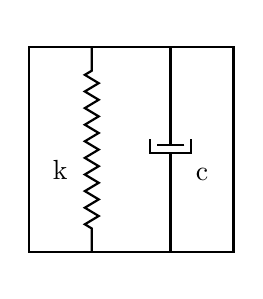
\begin{tikzpicture}[every node/.style={draw,outer sep=0pt,thick}]
\tikzstyle{spring}=[thick,decorate,decoration={zigzag,pre length=0.3cm,post length=0.3cm,segment length=6}]
\tikzstyle{damper}=[thick,decoration={markings,  
  mark connection node=dmp,
  mark=at position 0.5 with 
  {
    \node (dmp) [thick,inner sep=0pt,transform shape,rotate=-90,minimum width=15pt,minimum height=3pt,draw=none] {};
    \draw [thick] ($(dmp.north east)+(2pt,0)$) -- (dmp.south east) -- (dmp.south west) -- ($(dmp.north west)+(2pt,0)$);
    \draw [thick] ($(dmp.north)+(0,-5pt)$) -- ($(dmp.north)+(0,5pt)$);
  }
}, decorate]

\node (S) [minimum width=2.6cm,minimum height=2.6cm]{};
\node (sw_node) at (S.south) [draw=none,yshift=0cm,xshift=-0.5cm,anchor=north] {};
\node (nw_node) at (S.north) [draw=none,yshift=0.25cm,xshift=-0.5cm,anchor=north] {};
\draw [spring] (sw_node) -- (nw_node);
\node (k_node) at (sw_node) [draw=none,yshift=1.4cm,xshift=-0.4cm,anchor=north] {k};
\node (se_node) at (S.south) [draw=none,yshift=0cm,xshift=0.5cm,anchor=north] {};
\node (ne_node) at (S.north) [draw=none,yshift=0.25cm,xshift=0.5cm,anchor=north] {};
\draw [damper] (se_node) -- (ne_node);
\node (c_node) at (se_node) [draw=none,yshift=1.3cm,xshift=0.4cm,anchor=north] {c};

\end{tikzpicture}
\caption{Stiffener ($S$) Diagram}
\label{stiff}
\end{figure}

\begin{figure}	% rhos
 \centering
 \includegraphics[width=0.5\textwidth]{Figures/Q5_P1_RhoVectors.pdf}
 \caption{CoM and Rho Vectors}
 \label{rhos}
\end{figure}

\begin{figure}		% raytrace
\centering
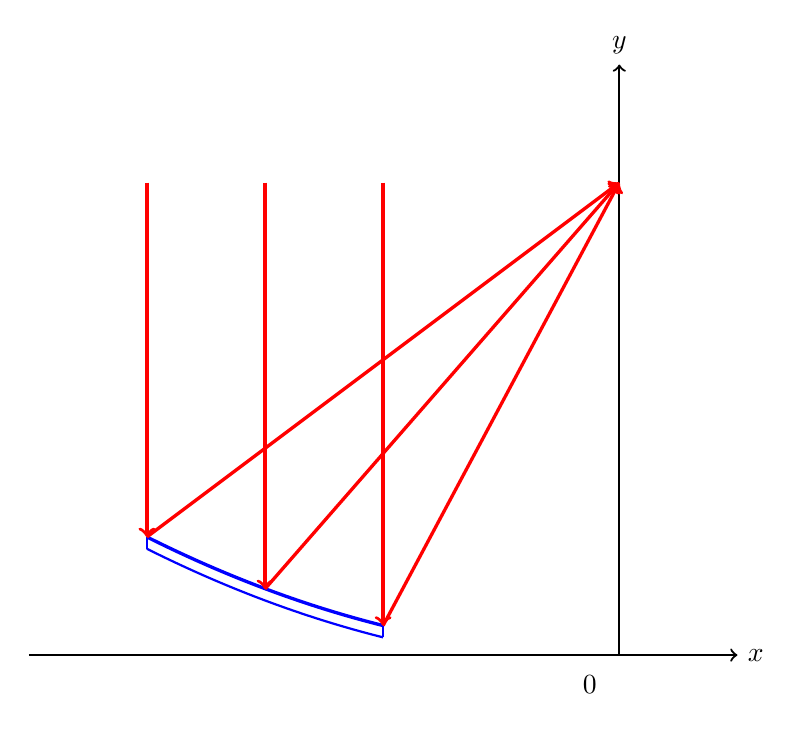
\begin{tikzpicture}[scale=1.5]
\def\f{4}
\def\xmin{-5} \def\xmax{1}
\def\ymin{0}  \def\ymax{5}
\def\fx{0} \def\fy{\f}
% draw axes
\draw (-.25,-.25) node[auto] {0};
\draw[->,thick] (\xmin,\ymin) -- (\xmax,\ymin) node[right] {$x$};
\draw[->,thick] (\ymin,\ymin) -- (\ymin,\ymax) node[above] {$y$};
% draw off-axis parabolic section
\draw[color=blue,very thick] plot [domain=-4:-2] (\x,{((\x)^2)/(4*\f)});
\draw[color=blue,thick] plot [domain=-4:-2] (\x,{((\x)^2)/(4*\f)-0.1});
\draw[-,color=blue,thick] (-4,{((-4)^2)/(4*\f)-0.1}) -- (-4,{((-4)^2)/(4*\f)});
\draw[-,color=blue,thick] (-2,{((-2)^2)/(4*\f)-0.1}) -- (-2,{((-2)^2)/(4*\f)});
% draw rays
\draw[->,color=red,very thick]  (-4,4) -- (-4,1); \draw[->,color=red,very thick]  (-4,1) -- (\fx,\fy);
\draw[->,color=red,very thick]  (-3,4) -- (-3,0.56); \draw[->,color=red,very thick]  (-3,0.56) -- (\fx,\fy);
\draw[->,color=red,very thick]  (-2,4) -- (-2,0.25); \draw[->,color=red,very thick]  (-2,0.25) -- (\fx,\fy);
\end{tikzpicture}
\caption{Nominal Raytrace}
\label{raytrace}
\end{figure}

 \subsection*{Objective}
 The objective of this analysis is to characterize the evolution of the focal point distribution when subjected to a random disturbance. This is accomplished by Monte Carlo Simulation (MCS) and an example based on user-defined values is presented in the results section. Furthermore, the functional dependence of the output distribution with respect to the input disturbance distribution is observed for a range user-defined values of the input distribution parameters and presented.
 
 % \subsection*{Assumptions}

% \begin{description}
	% \item[1)] The mirror section is an off-axis parabola.
	% \item[2)] All incoming plane waves focus to a single point.
	% \item[3)] The mirror surface is ideal and rigid.
	% \item[4)] The small angle approximation is valid for $\alpha$.
 % \end{description}
\section{Equations of Motion Derivation}

To derive the equations of motion, solve a force-balance for the kinetic equations, then use geometry to develop the kinematic equations and substitute these into the kinetic equations.

\subsection*{Kinetic Equations}

The kinetic equations are formulated by equating the free-body diagram (FBD) with the mass-acceleration diagram as shown in Figure~\ref{FBD=MAD}. The stiffening unit $x$- and $y$-force vector directions are determined by assuming the mirror is displaced in the positive respective direction with positive respective velocity, then inferring the restoring and resistive force imparted by each stiffening unit. The disturbance forces are defined as positive in the $+x$- and $+y$-directions. Referring to the stiffener diagram of Figure~\ref{stiff}, a force-balance for each identical unit as shown in Equation~\eqref{eq:stiffener} characterizes the reactive force at each node.

\begin{equation}
\label{eq:stiffener}
\begin{aligned}
		\sum{F} &= m\ddot{s}\\
		0 &= S - ks - c\dot{s}\\
		S &= ks + c\dot{s}
\end{aligned}
\end{equation}\

\begin{figure}	% FBD=MAD
 \centering
 \includegraphics[width=0.75\textwidth]{Figures/Q5_P1_FBD=MAD.pdf}
 \caption{Set the free-body diagram equal to the mass-acceleration diagram to formulate the kinetic equations}
 \label{FBD=MAD}
\end{figure}

\begin{subequations}
\label{eq:kinEQ}
\begin{align}
	\begin{split}
	\sum{F_x} &= m\ddot{x} \\
	m\ddot{x} &= -S_{x_1}-S_{x_2}+Dx \\
	m\ddot{x} &= -kx_1 - c\dot{x_1} - kx_2 - c\dot{x_2} + D_x \\
	\end{split}\\
	\begin{split}
	\sum{F_y} &= m\ddot{y}\\
	m\ddot{y} &= -S_{y_1}-S_{y_2}+Dx \\
	m\ddot{y} &= -ky_1 - c\dot{y_1} - ky_2 - c\dot{y_2} + D_y\\
	\end{split}\\
	\begin{split}
	\sum{M_G} &= I\ddot{\alpha}\\
	I\ddot{\alpha} &= \rho_{2_y}\left[-S_{x_2}+D_x\right] +  \rho_{2_x}\left[-S_{y_2}+D_y\right] + \rho_{y_1}S_{x_1} + \rho_{x_1}S_{y_1}  \\
	I\ddot{\alpha} &= \rho_{2_y}\left[-kx_2 - c\dot{x}_2+D_x\right] +  \rho_{2_x}\left[-ky_2 - c\dot{y}_2+D_y\right] + \rho_{1_y}\left[-kx_1 - c\dot{x}_1\right] + \rho_{1_x}\left[-ky_1 - c\dot{y}_1\right]  \\
	\end{split} \\ \nonumber
\end{align}
\end{subequations}

\subsection*{Kinematic Equations}

The kinematic equations define the interdependencies of the motion of the state variables. For this simulation, these are defined by the geometry of the mechanical system. Specifically, these equations define the positions and velocities of the mirror segment endpoints by the mirror segment CoM position, velocity, and rotation angle.

\begin{equation}
\label{eq:kinemEQ}
\begin{aligned}
		x_1 &= x - d\rho_{1_x} & x_2 &= x + d\rho_{2_x} \\
		\dot{x_1} &= \dot{x} - d\dot{\rho}_{1_x} & \dot{x_2} &= \dot{x} + d\dot{\rho}_{2_x} \\
		y_1 &= y - d\rho_{1_y} & y_2 &= y + d\rho_{2_y} \\
		\dot{y_1} &= \dot{y} - d\dot{\rho}_{1_y} & \dot{y_2} &= \dot{y} + d\dot{\rho}_{2_y}
\end{aligned}
\end{equation}

Where

\begin{equation}
\centering
	\begin{aligned}
	d\rho_{1_x} &= d\rho_1\cos\left( \phi_1 \right) & d\rho_{2_x} &= d\rho_2\cos\left( \phi_2 \right)\\
	d\dot{\rho}_{1_x} &= d\dot{\rho}_1\cos\left( \phi_1 \right) & d\dot{\rho}_{2_x} &= d\dot{\rho}_2\cos\left(\phi_2\right)\\
	d\rho_{1_y} &= d\rho_1\sin\left( \phi_1 \right) & d\rho_{2_y} &= d\rho_2\sin\left( \phi_2 \right)\\
	d\dot{\rho}_{1_y} &= d\dot{\rho}_1\sin\left( \phi_1 \right) & d\dot{\rho}_{2_y} &= d\dot{\rho}_2\sin\left(\phi_2\right)	
	\label{eq:drho}
	\end{aligned}
\end{equation}\

 For this simulation, all rotations about the CoM, $\alpha$, are small enough that the small-angle approximation, Equation~\eqref{eq:smallAngle}, is assumed valid.

\begin{equation}
\centering
	\begin{aligned}
	d\vec{\rho} &\approx \vec{\rho}\sin \left(\alpha\right) &\approx \vec{\rho}\alpha \\
	d\dot{\vec{\rho}} &\approx \vec{\rho} \left[d\left(\sin \left(\alpha\right)\right)\right] &\approx  \vec{\rho}\dot{\alpha}
	\label{eq:smallAngle}
	\end{aligned}
\end{equation}

Such that,

\begin{equation}
\centering
	\begin{aligned}
	d\rho_{1_x} &= \rho_1\alpha\cos\left( \phi_1 \right) & d\rho_{2_x} &= \rho_2\alpha\cos\left( \phi_2 \right)\\
	d\dot{\rho}_{1_x} &= \rho_1\dot{\alpha}\cos\left( \phi_1 \right) & d\dot{\rho}_{2_x} &= \rho_2\dot{\alpha}\cos\left( \phi_2 \right)\\
	d\rho_{1_y} &= \rho_1\alpha\sin\left( \phi_1 \right) & d\rho_{2_y} &= \rho_2\alpha\sin\left( \phi_2 \right)\\
	d\dot{\rho}_{1_y} &= \rho_1\dot{\alpha}\sin\left( \phi_1 \right) & d\dot{\rho}_{2_y} &= \rho_2\dot{\alpha}\sin\left( \phi_2 \right)
	\label{eq:drho}
	\end{aligned}
\end{equation}

The differential changes in position vectors, $d\rho_1$ and $d\rho_2$, are illustrated by Figures~\ref{drho12}.

\begin{figure}	% drho12
 \centering
 \subfigure[]{
 \includegraphics[width=0.6\textwidth]{Figures/Q5_P1_Rho1.pdf}}
 \subfigure[]{
 \includegraphics[width=0.5\textwidth]{Figures/Q5_P1_Rho2.pdf}}
 \caption{Rho Vectors}
 \label{drho12}
\end{figure}

\subsection*{Centroid Location}

Working with an off-axis parabolic mirror segment requires intermediate calculations to find the location of the centroid with respect to the vertex. The simulation presented assumes the $x$-coordinate of both mirror endpoints is known. First, calculate the arc length, $L$, of the mirror as follows.

\begin{equation}
\label{eq:arclength}
\centering
\begin{aligned}
	(dL)^2 &= (dx)^2 + (dy)^2 \\
	\frac{dL}{dx} &= \sqrt{1+\left(\frac{dy}{dx}\right)^2} \\
	L &= \bigintss_a^b \sqrt{1+\left(\frac{dy}{dx}\right)^2}dx
\end{aligned}
\end{equation}\

Then, find the mass of the mirror using a constant length density, $\rho_L$, and the arc length, $L$, between the known endpoint locations, $x_1$ and $x_2$.

\begin{equation}
\label{eq:mass}
\centering
\begin{aligned}
	m &= \rho_L L \\
	&= \rho_L \bigintss_{x_1}^{x_2} \sqrt{1+\left(\frac{dy}{dx}\right)^2}dx
\end{aligned}
\end{equation}\

Next, calculate the moments about the $x$- and $y$-axes. The moment is the mass of a differential element multiplied by the perpendicular distance from the axis.

\begin{equation}
\label{eq:moment1}
\centering
\begin{aligned}
	M_x &= \rho_L \bigintss_{x_1}^{x_2} y(x)\sqrt{1+\left(\frac{dy}{dx}\right)^2}dx \\
	M_y &= \rho_L \bigintss_{x_1}^{x_2} x\sqrt{1+\left(\frac{dy}{dx}\right)^2}dx
\end{aligned}
\end{equation}\

To calculate the centroid location, note that the moment about an axis is equal to the mass located at the centroid.\\

\begin{equation}
\label{eq:moment2}
\centering
\begin{aligned}
	M_x &= m\bar{y} \\
	M_y &= m\bar{x}
\end{aligned}
\end{equation}\

Thus,

\begin{equation}
\label{eq:centroid}
\centering
\begin{aligned}
	\bar{x} &= \frac{M_y}{m} \\
	&= \frac{\rho_L}{m} \bigintss_{x_1}^{x_2} x\sqrt{1+\left(\frac{dy}{dx}\right)^2}dx \\
	\\
	\bar{y} &= \frac{M_x}{m} \\
	&= \frac{\rho_L}{m} \bigintss_{x_1}^{x_2} y(x)\sqrt{1+\left(\frac{dy}{dx}\right)^2}dx
\end{aligned}
\end{equation}\

For a parabola,

\begin{equation}
\label{parabola}
\centering
\begin{aligned}
	y(x) &= \frac{1}{4f}x^2 \\
	\\
	\frac{dy}{dx} &= \frac{1}{2f}x
\end{aligned}
\end{equation}\\

$\vec{\rho}_V$, $\vec{\rho}_1$, and $\vec{\rho}_2$ of Figure~\ref{drho12} are easily calculated as the difference between the associated point position vectors.

\subsection*{Equations of Motion}

Substitute Equations~\eqref{eq:drho} into~\eqref{eq:kinemEQ}, then \eqref{eq:kinemEQ} into \eqref{eq:kinEQ} to generate equations of motion with $x$ and $y$ position of the CoM and $\alpha$ as the system states.

\begin{subequations}
\label{eq:fullEoM}
\centering
\begin{align}
	\ddot{x} &= \frac{1}{m}\left[-k\left(x - d\rho_{1_x}\right) -c\left(\dot{x} - d\dot{\rho}_{1_x}\right) - k\left(x - d\rho_{2_x}\right) -c\left(\dot{x} - d\dot{\rho}_{2_x}\right) + D_x \right]\\
	\nonumber \\
	\ddot{y} &= \frac{1}{m}\left[-k\left(y - d\rho_{1_y}\right) -c\left(\dot{y} - d\dot{\rho}_{1_y}\right) - k\left(y - d\rho_{2_y}\right) -c\left(\dot{y} - d\dot{\rho}_{2_y}\right) + D_y \right] \\
	\nonumber \\
	\begin{split}
	\ddot{\alpha} &= \frac{1}{I} \Biggl\{ \rho_{2_y}\left[-k\left(x - d\rho_{2_x}\right) - c\left(\dot{x} - d\dot{\rho}_{2_x}\right)+D_x\right] +  
													 \rho_{2_x}\left[-k\left(y - d\rho_{2_y}\right) - c\left(\dot{y} - d\dot{\rho}_{2_y}\right)+D_y\right]  \\
						&					  + \rho_{y_1}\left[-k\left(x - d\rho_{1_x}\right) - c\left(\dot{x} - d\dot{\rho}_{1_x}\right)\right] + 
													 \rho_{x_1}\left[-k\left(y - d\rho_{1_y}\right)  - c\left(\dot{y} - d\dot{\rho}_{1_y}\right)\right]  \Biggr\}
	\end{split}
\end{align}
\end{subequations}

\section{Simulation}

To simulate the dynamics of the mirror response, use MATLAB and generate random input disturbance vectors. The random disturbance, $\vec{D}$, is applied at the node \#2 (right) and given as Equation~\eqref{eq:dist}. The disturbance input is a force with random magnitude, $r$, and random direction, $\theta$, where $r \sim \mathcal{N}\left(r_0,\sigma_0\right)$ and $\theta \sim \mathcal{U}\left(0,2\pi\right)$. For this simulation, the input is an impulse at $t=0$, so the only non-zero value in the disturbance vector is at the initial state.\\

\begin{equation}
\label{eq:dist}
	\vec{D} = \left[
					\begin{array}{c}
					D_x\\
					D_y\\
					\end{array}
					\right]
				= \left[
					\begin{array}{c}
					r\cos{\theta}\\
					r\sin{\theta}\\
					\end{array}
					\right]
\end{equation}\\

 A first-order state-space representation of the equations of motion is integrated using \texttt{ODE45()} in MATLAB. Thus, for a realization of the random disturbance, a numerical deterministic solution of the mirror dynamics is obtained. The output is chosen to be the optical performance parameter of maximum spot size radius based on an exact raytrace. At each state, an exact raytrace as shown in a perturbed case by Figure~\ref{rt} is simulated in MATLAB using objects of \texttt{MirrorClass.m} and \texttt{RayClass.m}. In the focal plane, Figure~\ref{sd}, the maximum spot size radius is calculated as the euclidean norm of the chief ray intersection point with the intersection point of the ray farthest from the chief ray in the focal plane. The deviation of the chief ray intersection point from its nominal location is not considered. \\
 
 \begin{figure}	% rtsd
 \centering
 \subfigure[]{
 \includegraphics[width=0.45\textwidth,trim=1cm 6cm 2cm 6cm,clip]{Figures/Q5P1_raytrace.pdf}
 \label{rt}}
 \subfigure[]{
 \includegraphics[width=0.45\textwidth,trim=1cm 6cm 2cm 6cm,clip]{Figures/Q5P1_spotdiagram.pdf}
 \label{sd}}
 \caption{Raytrace (a) and corresponding detector plane spot diagram (b) for mirror in a perturbed state (rotation about the z-axis).}
 \label{rtsd}
\end{figure}
 
 When a Monte Carlo Simulation is run, a complete state history of the input and output are available for each realization and each combination of disturbance distribution parameters, $r_0$ and $\sigma_0$. The cost functional of each realization is the average of the maximum spot size radius at each state. A Gaussian distribution is assumed for the scalar output performance measure and the mean and standard deviation of this average are calculated for all realizations of a given distribution (i.e.\ $r_{ss_{max}} \sim \mathcal{N}\left(\mu_{out},\sigma_{out}\right)$ given $r_0$ and $\theta_0$). Thus, the output distribution parameters, $\mu_{out}$ and $\sigma_{out}$, are generated as a function of the input disturbance distribution parameters, $r_0$ and $\theta_0$.\\
 
 \subsection*{MATLAB Simulation Details}

\begin{sloppypar} 
The MATLAB simulation script first defines the geometric properties of the system. The function, \texttt{calcConicCentroid.m}, returns the indices of the centroid, point 1, and point 2 as well as the mass and moment of inertia of the parabolic mirror segment. Next, values are assigned to the spring rate and damping coefficient and the simulation time is specified. The MCS is accomplished by generating sample realizations of the disturbances, simulating mirror dynamics, and calculating the corresponding optical outputs a number of times for each disturbance distribution. Function \texttt{Q5\_Realization.m} returns the output dynamics and the spotsize for a given $r_0$ and $\sigma_0$, then the mean and standard deviation is computed for each combination. \\
 \end{sloppypar}
 
The function \texttt{Q5\_Realization.m} generates the random impulse disturbance based on the supplied distribution parameters. Function \texttt{state\_eqns.m} is supplied the time span, initial guess, and disturbance vector and the deterministic solution is computed by numerical integration of the first-order state equations using \texttt{ODE45.m}.From the output state vector, the mirror vertex position is calculated. The change in vertex position from the nominal location as well as the perturbed angle is passed to function \texttt{SingleMirror\_SpotSize.m}.\\
 
\texttt{SingleMirror\_SpotSize.m} defines properties of the mirror conic section and the direction of the input beam. Mirror objects are constructed from \texttt{MirrorClass.m} with the mirror properties and these mirror objects are used to construct ray objects from \texttt{RayClass.m}. Each ray object can be thought of as one complete trace of a ray through the optical system. It contains a segment for each propagation step and the coordinates of each endpoint of each segment. The class files \texttt{MirrorClass.m} and \texttt{RayClass.m} utilize and compliment work presented by Breckenridge and Redding.~\cite{RedBreck} The final surface in the raytrace is the reference surface and the intersection point of the rays with that plane defines the spot diagram. \texttt{SingleMirror\_SpotSize.m} finishes by calculating the distance between the chief ray and each of the marginal ray reference surface intersection points and determines the maximum distance. This maximum distance is defined as the spot size for this analysis.After all realizations have run and the distribution of the output has been calculated, the results are plotted.

 \section{Results}

The resulting motion caused by one realization of the input disturbance is plotted in Figure~\ref{motionPlots}. It can be seen the disturbance is an impulse and the resulting motion is stable, settling back to the equilibrium point. Figure~\ref{ssEvolution} depicts the evolution of the maximum radius of the spot size during the simulation. The spot size radius is a positive definite quantity and the average spot size over the simulation time is the output metric.\\

\begin{figure}
	\centering
	\subfigure[]{
	\includegraphics[width=0.45\textwidth,trim=0.8cm 6cm 2cm 6cm,clip]{Figures/Q5P1_real_Disturbance.pdf}}
	\subfigure[]{
	\includegraphics[width=0.45\textwidth,trim=0.8cm 6cm 2cm 6cm,clip]{Figures/Q5P1_real_CoM_Motion.pdf}}
	\subfigure[]{
	\includegraphics[width=0.45\textwidth,trim=0.8cm 6cm 2cm 6cm,clip]{Figures/Q5P1_real_CoM_LinDisp.pdf}}
	\subfigure[]{
	\includegraphics[width=0.45\textwidth,trim=0.8cm 6cm 2cm 6cm,clip]{Figures/Q5P1_real_CoM_AngDisp.pdf}}
	\caption{Dynamic responses to force disturbance. (a) Impulse force disturbance input at node \#2. (b) CoM motion. (c) CoM linear displacements. (d) Mirror angular displacement.}
	\label{motionPlots}
\end{figure}

\begin{figure}
	\centering
	\includegraphics[width=0.65\textwidth,trim=1cm 6cm 2cm 6cm,clip]{Figures/Q5P1_real_SpotSizeEvolution.pdf}
	\caption{Detector plane maximum spot size radius evolution for a single realization.}
	\label{ssEvolution}
\end{figure}


MCS with random input disturbance realizations generate a sufficient number of output data sets for which the distribution parameters, $\mu_{out}$ and $\sigma_{out}$, are computed. These output distributions are then generated for varied user-supplied values of the input distribution parameters, $r_0$ and $\sigma_0$. Figures~\ref{distrel} are plots of the input to output statistics relationships. Analysis of these plots validates some intuition regarding the simulation. Figure~\ref{mu_v_r0} reveals a linear increase in the mean of the average spot size as the mean strength of the input disturbance is increased. Naturally, a larger disturbance generates a greater misalignment and poorer optical performance. Similarly, Figure~\ref{sigma_v_r0} shows a linear increase in the mean of input disturbance promotes an increase in the standard deviation of the average spot size. Figure~\ref{mu_v_sigma0} indicates that an increase in the standard deviation of the input disturbance does not noticeably change the mean of the average spot size except for zero-mean input. This observation suggests that the assumption of a Gaussian distribution of the output is appropriate because the distribution about the mean input mimics to the distribution about the mean output. Figure~\ref{sigma_v_sigma0} reveals an expected result in that the standard deviation about the mean output increases with the standard deviation of the input disturbance. \\

\begin{figure}
	\centering
	\subfigure[]{
	\includegraphics[width=0.45\textwidth,trim=0.8cm 6cm 2cm 6cm,clip]{Figures/Q5P1_stat_mu_v_r0.pdf}
	\label{mu_v_r0}}
	\subfigure[]{
	\includegraphics[width=0.45\textwidth,trim=0.8cm 6cm 2cm 6cm,clip]{Figures/Q5P1_stat_mu_v_sigma0.pdf}
	\label{mu_v_sigma0}}
	\subfigure[]{
	\includegraphics[width=0.45\textwidth,trim=0.8cm 6cm 2cm 6cm,clip]{Figures/Q5P1_stat_sigma_v_r0.pdf}
	\label{sigma_v_r0}}
	\subfigure[]{
	\includegraphics[width=0.45\textwidth,trim=0.8cm 6cm 2cm 6cm,clip]{Figures/Q5P1_stat_sigma_v_sigma0.pdf}
	\label{sigma_v_sigma0}}
	\caption{Distribution parameter relationships}
	\label{distrel}
\end{figure}


\input{6-conclusion}
\bibliographystyle{aiaa}
\bibliography{ref}
\end{document}
